\documentclass[12pt, twoside]{report}
\usepackage[utf8]{inputenc}
\usepackage[a4paper, top=30mm, left=20mm, bottom=20mm,
    right=20mm]{geometry}
\usepackage[dvipsnames]{xcolor}
\usepackage{graphicx}
\usepackage{color}
\usepackage{fancyhdr}
\fancyhead[LO,RE]{\itshape \nouppercase Chapter \arabic{chapter}}
\usepackage{amssymb}
\usepackage{csquotes}
\usepackage{amsmath}
\usepackage{amsthm}
\usepackage{mathtools} % shortintertext
\usepackage{faktor}
\usepackage[backend=bibtex, 
            maxbibnames=10,
            style=alphabetic]{biblatex}
\usepackage{hyperref}
\usepackage{subfigure}
\usepackage[font={small,it}]{caption}
\usepackage{algpseudocode}
\usepackage[plain]{algorithm}
\usepackage[shortlabels]{enumitem}
\usepackage{booktabs}
\usepackage{mhchem} % chemical reactions
\usepackage{cleveref} % multireference (eq 1.2-1.5)
\usepackage{pgfgantt} % nice Gantt diagrams


\pagestyle{fancy}

% Images path
\graphicspath{ {img/} }

% ABNT foreign words should be in italic
\newcommand{\foreignword}[1]{\textit{#1}}
\newcommand{\toolname}[1]{\textit{#1}}
\newcommand{\fieldR}{\mathbb{R}}
\newcommand{\powerset}{\mathcal{P}}
\newcommand{\probability}{\mathbb{P}}
\newcommand{\expectation}{\mathbb{E}}
\newcommand{\algname}[1]{\texttt{#1}}
\newcommand{\langname}[1]{\texttt{#1}}
\newcommand{\varname}[1]{\texttt{#1}}
\newcommand{\floor}[1]{\lfloor #1 \rfloor}
\newcommand{\ceil}[1]{\lceil #1 \rceil}
\newcommand{\mathsc}[1]{{\normalfont\textsc{#1}}}
\newcommand{\forest}{\mathcal{F}}
\newcommand{\pfsnode}[1]{\mathbf #1}
\newcommand{\species}[1]{\textit{#1}}
\newcommand{\gender}[1]{\textit{#1}}

% remove returns of the same line in pseudocodes
\algrenewcommand\Return{\State \algorithmicreturn{} } 

\DeclareMathOperator*{\argmin}{argmin} 

\addbibresource{references.bib}

\newtheorem{mydefinition}{Definition}
\numberwithin{mydefinition}{section}
\newtheorem{mytheorem}{Theorem}
\numberwithin{mytheorem}{section}
\newtheorem{mylemma}{Lemma}
\numberwithin{mylemma}{section}
\newtheorem{corollary}{Corollary}
\numberwithin{corollary}{section}


\begin{document}
\pagenumbering{roman}
\thispagestyle{empty}
\begin{center}
{\Large
{\bf Identification of cell signaling pathways based on biochemical 
    reaction kinetics repositories}\\
\bigskip
\bigskip
\bigskip
\bigskip
    {\bf \href{mailto:gustavo.estrela.matos@gmail.com}{Gustavo Estrela de Matos}}\\
\bigskip
\bigskip
\bigskip
\bigskip
\textsc{
    Text presented\\[-0.25cm] 
    to\\[-0.25cm]
    Institute of Mathematics and Statistics\\[-0.25cm]
    of the\\[-0.25cm]
    University of São Paulo\\[-0.25cm]
    For\\[-0.25cm]
    The Qualification Exam Of Master Of Science\\
    }
\bigskip
\bigskip
\bigskip
\bigskip
Field of knowledge: Computer Science\\
\bigskip
Advisor: Dr. Marcelo da Silva Reis\\
\bigskip
\bigskip
\bigskip
\bigskip
\bigskip
\bigskip
\bigskip
\bigskip
Center of Toxins, Immune-Response and Cell Signaling (CeTICS)\\
\bigskip
Special Laboratory of Cell Cycle, Butantan Institute\\
\bigskip
\bigskip
{\normalsize During the development of this work the author received 
    financial support from FAPESP.}\\
\bigskip
\bigskip
\bigskip
São Paulo, \today
}
\end{center}
\newpage

\chapter*{Abstract}
Cell signaling pathways are composed of a set of biochemical reactions 
that are associated with signal transmission within the cell and its 
surroundings. Traditionally, these pathways are identified through 
statistical analyses on results from biological assays, in which 
involved chemical species are quantified. However, once generally it is 
measured only a few time points for a fraction of the chemical species, 
to effectively tackle this problem it is required to design and simulate 
functional dynamic models. Recently, it was introduced a method to 
design functional models, which is based on systematic modifications of 
an initial model through the inclusion of biochemical reactions, which 
in turn were obtained from the interactome repository KEGG. 
Nevertheless, this method presents some shortcomings that impair the 
estimated model; among them are the incompleteness of the information 
extracted from KEGG, the absence of rate constants, the usage of 
sub-optimal search algorithms and an unsatisfactory overfitting 
penalization. In this project, we propose a new methodology for 
identification of cell signaling pathways, which will make use of a 
myriad of public interactome and biochemical reaction kinetics 
repositories to deal with the incompleteness of a priori information. 
Moreover, we will use optimal algorithms for model selection, as well as 
more effective cost functions for overfitting penalization. The new 
methodology will be tested on artificial instances and also on cell 
signaling pathways identification in our case study, the Y1 mouse 
adrenocortical tumor cell line. (AU)
 
\tableofcontents

\clearpage
\pagenumbering{arabic} 

\nocite{*}
\chapter{Introduction}
\label{chap:intro}
%begin-include
% TODO: remove all contractions and spelling errors

% Outline of this section
% First we should start with a two-page description of the project with:
% - What are cell signaling pathways
% - What types of computational models we have for these pathways and 
% which one do we use
% - What can we do with those networks and how hard is it to get one to 
% work
% - What are the basic tasks to build a pathway
% - What has Lulu done and what are the limitations of her work
% - How do we intend to surmount those limitations


% Subsection Then we should state the main objectives/challenges of our 
% work
% Subsection Then we should give a short description of the work 


% What are cell signaling pathways and how is it important to study them
% - control how cell behaves in different types of environments
% - cancer cells have bad behavior
% - that's one reason to study signaling networks
Cell Signaling pathways are cascades of chemical interactions that 
allow the communication between the cell environment and the 
cell itself. These pathways are also able to regulate many cell 
functions, including DNA replication, cell division and cell death. We
can observe the functioning of signaling pathways as a mechanism that 
can conform the cell behavior with signals that come from the 
environment conditions in which the cell is placed. The studies of cell 
signaling pathways can lead to determining how cells can respond to 
different stimuli; for instance, with the studies of signaling pathways
activated by a chemical species, one could determine how an unhealthy 
cell would respond to a drug containing this species.

% There are computational models for signaling networks
% - Michaelis Menten equations for chemical interactions
% - With a system of ODES we can then simulate the cell behavior
% - However, the huge number of interactions happening in the cell makes
%   it impossible to consider everything.
% - Therefore we must know 
It's possible to construct mathematical models to represent a set of
chemical reactions and consequently a signaling network. One approach on 
the modeling of those interactions is based on the law of mass action. 
This law proposes that the rate of a chemical reaction is proportional 
to the product of reactants concentrations, i.e we can calculate the 
concentration change rate of a species in an interaction by calculating 
the product of reactants concentrations, up to a multiplying constant. 
If we consider the set of interactions of a signaling pathway, we can
then come up with a system of ordinary differential equations (ODEs) 
that can model the dynamics of the concentration of each chemical 
species from the pathway. Generally, these systems are complex and 
cumbersome, if not impossible, to be solved analytically, therefore we 
resort on computational models that apply numerical methods to 
approximate solutions of these systems.

% How do we create these computational models and what should they do?
In this work, we are interested in computational models that can 
reproduce the behavior of signaling networks, comparing experimental 
measures---generally based on Western blot data---to simulated results.
The figure~\ref{fig:signal_pathway_example} shows a set of interactions
as well as parameters of a model of a signaling network. To create these 
computational models, two main tasks need to be accomplished.

\begin{figure}[!ht]
\centering 
    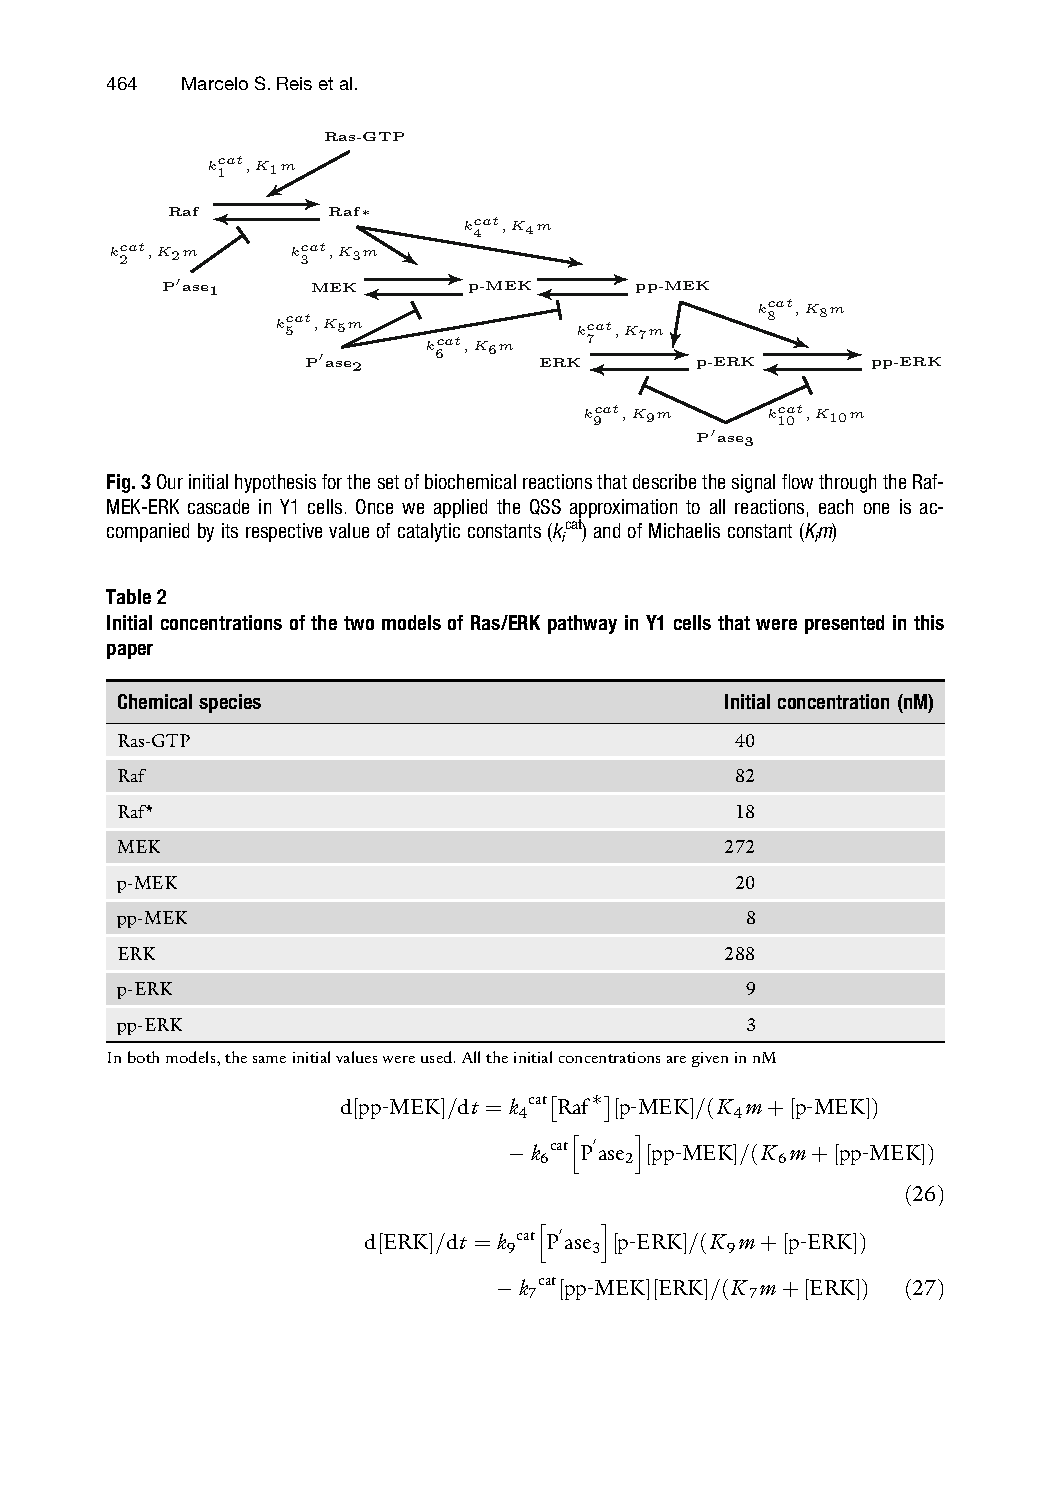
\includegraphics[width=\textwidth, viewport=40 500 460 660, clip]{introduction/signal_pathway_example_full_page.pdf}
\caption{The above diagram show a hypothesis for a signaling pathway 
    that flows through Raf-MEK-ERK cascade. Names in bold represent 
    chemical species. Names in italic represent parameters of the 
    ordinary differential equation of each interaction.Horizontal arrows
    represent phosphorylation when directed from left to right or 
    dephosphorilation when directed in the opposite direction. Other 
    arrows represent positive feedback if they are directed downwards or 
    negative feedback otherwise. Image copied from Marcelo S. Reis et.
    al (2017)~\cite{Reis2017}.}
\label{fig:signal_pathway_example}
\end{figure}

The first task one must complete to create a model is to determine a set 
of interactions to consider in the ODE system. Searching for pathway maps
on the Kyoto Encyclopedia of Genes and Genomes 
(KEGG)~\cite{Kanehisa2000kegg} is a good start. The KEGG PATHWAY 
Database provides manually drawn diagrams that represent signaling 
networks created with experimental evidences. However, it's possible 
that there's no pathway on KEGG that is able to correctly represent the 
biological experiment of interest; for those situations, it's necessary 
to modify the pathway by adding or even removing interactions. One might 
reason that we should use as many interactions as we can to get a better 
simulation, however, this usually implies in poor or computationally 
infeasible models because of two reasons: first, complex models will 
require more time in the numerical solution computation, which may be 
infeasible due to limited computational resources; and second, when 
considering many interactions, we are also placing many parameters 
(multiplying constants of the differential equations) on the model, and 
finding appropriate values for them becomes harder as we increase the 
number of parameters.

The second task to create a model is to find values for all the system
parameters. There are two approaches for this task, you can either 
fetch values for these constants from the literature or you can find 
values that makes the model output approximate the experimental 
observations. For the first approach, repositories such as 
BioModels~\cite{le2006biomodels} can be used; for the second approach, 
statistical and optimization methods can be used. For optimization, it 
is necessary to define a metric that can evaluate how close the 
parameters brings the model output to the experimental observation so
that you can search for the optimal parameter in the parameter space. 
Statistical inference, in the other hand, usually tries to maximize some 
likelihood function, which is defined to represent the probability of a 
model, with a set of parameter values, to reproduce the experimental 
observation.

% However, we might have missed some interactions or even added irrelevant ones
After completing both tasks, however, as we mentioned before, we might 
still not have found a model that fairly approximates the biological 
experiment of interest. That could indicate that the set of chemical 
interactions chosen for the model is incomplete or has interactions that
are not relevant for the biological experiment. Therefore, it is 
desirable to construct a systematic method of modifying the set of 
chemical reactions in order to find the optimal set.

% Lulu solved it as a combinatorial problem
With the title ``A method to modify molecular signaling networks through
examination of interactome databases"~\cite{Wu15} Lulu Wu presented in 
her masters dissertation a methodology to systematically modify 
computational models of signaling networks to better simulate biological 
experiments. Starting with a model that does not approximate well the 
biological data, this methodology proposes to add a set of interactions
to the model topology in order to better simulate the signaling pathway 
of interest. This set of interactions is a subset of interactions from a 
database created by Lulu Wu, joining information
from many static maps available on KEGG. The choice of this subset can 
be modeled as a combinatorial optimization problem in which the search 
space is the set of all possible subsets of interactions to be added.
The cost function of this problem, however, is not as simple to define 
as the search space. Note that the search space itself does not define 
models, but only the topology, i.e. the set of interactions, therefore, 
to consider the second task of creating computational models for 
signaling networks, the cost function must take into account the set of 
values for the model parameters. As an example, we could define the cost 
as the minimum distance between model and experimental measures 
considering all possibilities of parameter values; however, 
unfortunately, finding the minimizing parameter values is a hard 
problem.

Since this is a hard problem, the method presented by Lulu Wu 
implements a heuristic version of this cost function. This heuristics 
is based on a Simulated Annealing procedure that searches for a set of 
parameter values trying to minimize (as much as possible) the distance 
between model and experimental measures; the best found distance is then
considered as the cost of the model. Once the number of possible model 
topologies grows exponentially on the number of interactions from the 
database, the algorithm used to traverse the search space of subset of 
interactions is also a heuristic, and it is based on the greedy 
algorithm called Sequential Forward Selection (SFS)~\cite{Whitney1971}.
The heuristic implemented by Lulu Wu selects a fixed number of 
interactions from the database and then creates candidate models by 
adding to the current solution the respective interaction; then, after 
evaluating the cost function for each model, the algorithm moves to the 
best candidate.

%The work of Lulu Wu was succesful on 

% Her work however had a few flaws...
% To surmount these limitations
% - gather information from many data sources
% - create new search algorithms
% - use Bayesian approach 


\chapter{Fundamental Concepts}
\label{chap:fundamental_concepts}
%begin-include

In this section we provide the concepts that are fundamental to 
understand the biological and computational problems, methodologies and
results that we will present in this work. We start this chapter 
presenting what is a cell signaling pathway and how can one take 
measures to identify its activity on the cell. Later we present how 
it is possible to represent chemical iteractions as differential 
equations, and how that allows one to model a cell signaling pathway
with a system of ordinary differential equations. Then, we present 
more formally the problem we are trying to solve on this project, the
identification of cell signaling pathways, as well as the state of the
art methods of model ranking. Finally, we present the basics of 
posterior distribution sampling, which is a useful tool when working 
with Bayesian approaches, such as the ones used on this project to rank 
models.

% What I want to talk about in this section?
% - Cells signaling pathways are part of the cell communication system,
% and it allows the cell to perceive the conditions of the environment 
% and also to change its behaviour according to the input signal.
% - The signals perceived by a cell can come from cells that very close
% (including itself), as in synapses or it can travel long distances in 
% the organism, as in hormones.
% - When a signal reaches a cell, it can either activate a receptor in
% the cell membrane or diffuse into the cell.
% - Once this happen, the signal or the activated receptor can trigger
% a sequence of chemical interaction, altering the conformation and 
% state of proteins and also changing the concentration of chemical 
% species in the cell. Ultimately, this chain of effects can alter the 
% behaviour of the cell, what is called signal transduction.
% - Studying signaling pathways is important because they help us 
% understand the mechanisms of a cell, which can for example, elucidate 
% treatments for diseases.
\section{Cell Signaling Pathways}
Cell signaling pathways are part of the complex cell communication 
system, and it allows the cell to perceive the conditions of the 
environment in which it is placed and change its behaviour accordingly.
Signaling pathways participate in the regulation of many cell functions,
including development, division and cell death~\cite{Hancock2017}. The
dynamic of a signaling pathway can also be releated to diseases, as in
many cases of cancer.

The signal perceived by a cell can come from cells that are close 
(including the same cell that produced the signal), as in synapses, or 
it can travel long distances in the organism, as in hormones. When a 
signal reaches a cell, it binds to a specific receptor in the membrane,
and once that happens, the receptor can trigger a sequence of chemical 
interactions that can include change of conformation of proteins, 
activation or inactivation of proteins, and change of concentration of
chemical species in the cell. Ultimately, this chain of chemical 
reactions caused by the signal can alter the behaviour of the cell, what 
is called signal transduction.

Since signaling pathways participate in many of the cell functions, and 
are also related to diseases, it is important to study those structures
in order to get a better understanding of the cell mechanisms and 
diseases. One approach on the study of the cell signaling pathways is to 
measure the concentration change of proteins and how they interact to
produce those changes.

% - Western blot is a technique that can indicate the amount of a 
% specific protein that is in a mixture of proteins
% - This technique shows the presence of a protein in a mixture by 
% ``blotting'' these molecules into a membrane. 
% - Repeating the procedure in different times define time-course 
% observations of the protein in a biological experiment.
% - With these observations in hand, the researcher is able to construct 
% a measurement that is relevant to describe the biological experiment. 
% For instance, in a signaling network where a protein is closely 
% related to the behaviour of interest of the cell, this protein is a 
% good candidate as a measure of the system.
\section{Measurements of Proteins in Cell Signaling Pathways}
Western blot~\cite{Towbin1979} is a laboratory technique that can 
indicate the amount of a specific protein that is present in a mixture. 
This technique shows the presence of a protein in a mixture by 
``blotting'' a membrane where the molecules of interest are located. We 
can summarize the procedure in the following steps: first a mixture 
containing a sample of cells of interest must be created; 
second, proteins from the mixture should be fixed on the blotting 
membrane; third, an antibody should bind to the target protein 
molecules; and finally, a method for highlighting the bound antibody 
should be applied. An image of the resulting membrane can then be 
analyzed with computer programs to quantify the relative concentration 
(with respect to some other protein, usually a control protein that has 
fairly the same concentration during the whole experiment) of the 
protein of interest.

By repeating this procedure in different times it is possible to create 
time-course observations of proteins throughout the biological 
experiment. With this tool, a researcher can choose a set of relevant 
proteins from a signaling network and gain knowledge about the dynamics 
of such chemical species during the experiment. For instance, in a 
signaling network experiment in which it is desired to understand how
the change of concentrations of a species at the beginning of the 
pathway changes the concentration of some species at the end of the 
cascade, then measurements of both are relevant to understand the 
biological experiment. Figure~\ref{fig:western_blot_example} presents an 
example of time-course Western blot for an experiment where it is 
desirable to understand how extracellular signal-regulated kinase (ERK)
is activated (phosphorylated) as a function of levels of Rat sarcoma
bound to guanosine triphosphate (Ras-GTP).

\begin{figure}[!ht]
\centering
    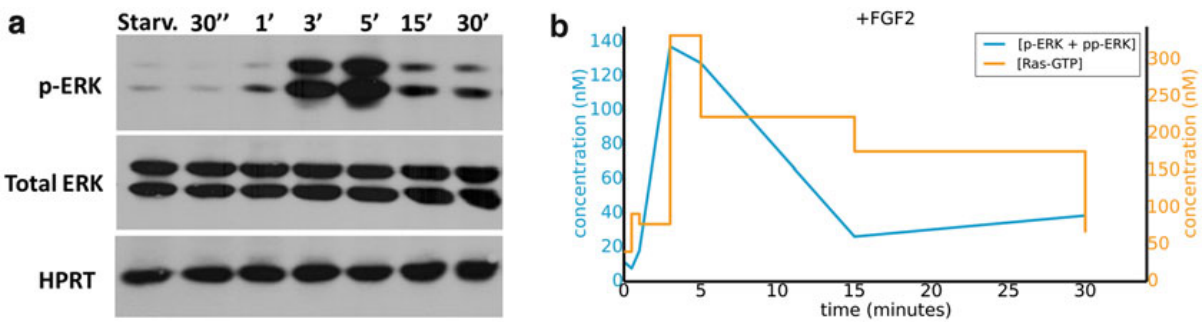
\includegraphics[width=\textwidth]{fundamental_concepts/western_blot.png}
    \caption{Figure {\bf a} shows time-course measurements of ERK, 
    phosphorylated ERK (p-ERK) and hypoxanthine-guanine 
    phosphoribosyltransferase (HPRT). HPRT is a ``loading'' protein, 
    that means that its concentration is fairly the same through the 
    experiment, and therefore it is used as a normalizing factor to 
    total ERK concentration. Figure  {\bf b} shows values of 
    phosphorylated ERK that are obtained after processing Figure 
    {\bf a}. Original image of Marcelo S. Reis et al. 
    (2017)~\cite{Reis2017}.}
    \label{fig:western_blot_example}
\end{figure}

These measurements alone do not always provide means for researchers to 
understand a cell signaling pathway experiment. However, if we create a 
computational model for this signaling networks that is able to 
reproduce experimental data, then we might use this model as a 
summary of the signaling network, which can provide to researchers 
evidences of the biological phenomena.


% What do I need to talk about?
% - We can model the concentration changes of chemical species as 
% differential equations, using the mass-action kinetic laws
% - The mass action kinetic law states that in an elementary reaction,
% the rate of a chemical reaction is directly proportional to the 
% product of the reactants concentrations.
% - What is elementary?
% 2.1 Elementary reactions rate equations
% - Types of elementary: first order reaction and second order reaction
% - How do we write up these two? 
% - Chemical notation with constants
% - From there we can write a system of differential equations to 
% describe the signaling pathway.
% - As an example, let's show the equations for a simple enzymatic 
% equation.
% 2.2 Simplifications of reactions
% - More can be done. We can simplify some equations 
% 2.1 Mass conservation simplification
% 2.2
\section{Dynamic Modeling of Cell Signaling Pathways}
One approach onto modeling cell signaling pathways is to model the 
dynamics of the concentrations of chemical species involved. This can be
accomplished when using the law of mass action~\cite{Voet2010}. This law 
states that, in an elementary reaction, the speed (or rate) of a 
chemical reaction is proportional to the product of the concentration of 
all reactants. An elementary reaction is a reaction in which there is no 
participation or need of an intermediate reaction to describe the first 
in a molecular level. In practice, it is more common to see two types of 
elementary reactions, they are first or second order reactions. 

\subsection{Modeling Elementary Reaction Rates}
A first order reaction is composed of one reactant only. Suppose A is 
the only reactant and B is the only product of a reaction, then we can
write this reaction as:
\begin{equation*}
\ce{
    A -> B
}.
\end{equation*}
The reaction rate of this reaction, according to the law of mass 
action, is 
\begin{equation*}
    k_1[\text{A}],
\end{equation*}
where $k_1$ is some constant and [A] is the concentration of A. It is
import to note that the constant $k_1$ is a rate coefficient of the 
reaction and, therefore, it can only assume positive values.

A second order reaction is composed of two reactants. Suppose C and D 
are both and the only reactants and F is the product of a reaction, then
we can write this reaction as:
\begin{equation*}
\ce{
    C + D -> F
}.
\end{equation*}
The reaction rate of this reaction is:
\begin{equation*}
    k_2\text{[C][D]},
\end{equation*}
where $k_2$ is a (positive) constant and [C] and [D] are the 
concentrations of C and D, respectively.

Using these two laws to calculate the speed of reactions, we are able 
to describe how the concentration of chemical species in a system change 
through time using differential equations. To illustrate this and future 
concepts of this section, we are going to consider a minimal system 
composed of a simple enzymatic reaction:
\begin{equation}
\ce{
    E + S <=>[\ce{$k$_f}][\ce{$k$_r}] ES ->[\ce{$k_{cat}$}] E + P
},
\label{eq:simple_enzymatic}
\end{equation}
where E is an enzyme, S is a substrate, ES is the enzyme-substrate
complex, and P is the product.

Each arrow in Equation~\ref{eq:simple_enzymatic} represents one 
elementary reaction, and the names over or under arrows represent 
reaction rate constants. All three reactions can be represented by the
equations:

%The first reaction has E and S as reactants and
%ES as a product, and can be written as 
\begin{subequations}
\begin{align}
\ce{
    E + S ->[\ce{$k_f$}] ES 
} \label{eq:es_complex_fwd} \\
\ce{
    ES ->[$k_r$] E + S
} \label{eq:es_complex_rev} \\
\ce{
    ES ->[$k_{cat}$] E + P
} \label{eq:es_pe} 
\end{align}
\end{subequations}
and they have, respectively, reaction rates of:
\begin{equation*}
\begin{aligned}
    & k_f\text{[E][S]} \\
    & k_r\text{[ES]} \\
    & k_{cat}\text{[ES]}.
\end{aligned}
\end{equation*}

Now, to determine a model of the concentration dynamics for
Reaction~\ref{eq:simple_enzymatic}, we will write a system of ordinary
differential equations. To do so, we should take every chemical species 
and calculate its concentration change rate based on the rate of each 
reaction that it participates. For instance, the enzyme E is a 
reactant on Reaction~\ref{eq:es_complex_fwd} and is also a product on 
reactions~\ref{eq:es_complex_rev} and~\ref{eq:es_pe}, then we consider 
that E changes its concentration over time ($t$) according to the 
differential equation:
\begin{equation}
    \frac{d[\text{E}]}{dt} = -k_f\text{[E][S]} + (k_r + k_{cat}) \text{[ES]}
\end{equation} 
Note that we are adding reation rates in which the species is a product
and we are subtracting reaction rates in which the species is a
reactant. Repeating this procedure for every other species of the 
enzymatic reaction leads to the following system of ordinary 
differential equations:
\begin{subequations}
    \label{eq:full_system}
    \begin{align}
        \frac{d[\text{E}]}{dt} & =  
            -k_f\text{[E][S]} + (k_r + k_{cat}) \text{[ES]} 
            \label{eq:dEdt} \\
        \frac{d[\text{S}]}{dt}  & = 
            -k_f\text{[E][S]} + k_r\text{[ES]} 
            \label{eq:dSdt} \\
        \frac{d[\text{ES}]}{dt} & =  
            k_f\text{[E][S]} - (k_r + k_{cat}) \text{[ES]} 
            \label{eq:dESdt} \\
        \frac{d[\text{P}]}{dt} & = k_{cat}\text{[ES]} \label{eq:dPdt}.
    \end{align}
\end{subequations}

% Ok, what do I really want to talk about here: Michaelis Menten 
% simplification of enzymtic reactions
% - Before anything, we should use mass conservation to produce the 
% d[ES]/dt equation.
% - Then we should mention the steady-state proposal of Michaelis Menten
%   -> should I use a picture? Maybe I can compare two initial states,
%      one with [S] >> [E] and the other not.
% - Mention that we can suppress a lot of parameters with this 
%   simplification
\subsection{Simplification of Dynamic Models}
The System~\ref{eq:full_system} can be simplified if we
apply properties of enzymatic reactions together with algebraic 
simplifications. We will show then how to derive the quasi-steady-state 
Michaelis-Menten model for enzymatic reactions. With the correct 
assumptions, this model is able to reproduce the behaviour of an 
enzymatic reaction without considering the intermediate enzyme-substrate 
complex.

A basic the principle we need to apply to our system in order to derive
the Michaelis-Menten model is the principle of mass conservation. This 
principle is valid if we assume that the 
reactions~\ref{eq:simple_enzymatic} are isolated, meaning that the 
chemicals on these reactions are not involved in other reactions at the
same time. Applying this principle to the enzyme chemical, produces the
following equation:
\begin{equation*}
    \text{[E$_0$]} = \text{[E] + [ES]}.
    \label{eq:E_conservation}
\end{equation*}
If we apply this equation to the derivative of the concentration of ES,
we will get the following equation:
\begin{equation}
    \frac{d[\text{ES}]}{dt} =  
        k_f(\text{[E$_0$]} - \text{[ES]})\text{[S]} 
        - (k_r + k_{cat}) \text{[ES]}. 
        \label{eq:dESdt_2}
\end{equation}

One more assumption is necessary to derive the simplification. This 
assumption states that the concentration of substrate-enzyme complex
does not change over time, i.e. $\frac{d[\text{ES}]}{dt} = 0$, and it 
was first proposed in 1925 by Briggs and Haldane~\cite{Briggs1925}. 
Generally, this assumption is applicable whenever [S] $\gg$ [E]. 
Applying this assumption together with the mass conservation assumption 
on the Equation~\ref{eq:dESdt_2}, we get:
\begin{equation*}  
    \begin{aligned}
        \text{[ES]} (k_r + k_{cat}) &= 
            k_f(\text{[E$_0$]} - \text{[ES]})\text{[S]}, \\
        \text{[ES]} &= \frac{\text{[E]}_0\text{[S]}}{K_m + \text{[S]}}, 
    \end{aligned}
\end{equation*}
in which $K_m = \frac{k_{cat} + k_r}{k_f}$ is known as Michaelis 
constant. Considering this, we can rewrite the rate of [P] as:
\begin{equation}
    \frac{d\text{[P]}}{dt} = k_{cat}\frac{\text{[E]}_0\text{[S]}}
        {K_m + \text{[S]}}.
    \label{eq:dPdt_2}
\end{equation}
And finally, if we apply mass conservation to the substrate, we will get
the following equation:
\begin{equation*}
    \text{[S$_0$]} = \text{[S] + [ES] + [P]},
\end{equation*}
then, we can differentiate this equation on $t$ and use the 
quasi-steady-state assumption ($\frac{d\text{[ES]}}{dt} = 0$) to obtain:
\begin{equation}
    \frac{d\text{[S]}}{dt} = - \frac{d\text{[P]}}{dt}.
    \label{eq:dSdt_2}
\end{equation}

Now, with equations~\ref{eq:dPdt_2}~and~\ref{eq:dSdt_2} we are able to
reproduce the dynamics of the substrate and product of the enzymatic 
reaction. Therefore, using the Michaelis-Menten model, we could simplify 
the System\ref{eq:full_system} that had four equations and three 
parameters to a new model that has only two equation and two parameters 
($k_{cat}$ and $K_m$). Figure~\ref{fig:michaelis_menten} shows a 
comparison between the complete and Michaelis-Menten models of enzymatic 
reactions.

\begin{figure}[H]
  \centering 
  \begin{tabular}{c c}
    \subfigure[] {\scalebox{1}{
    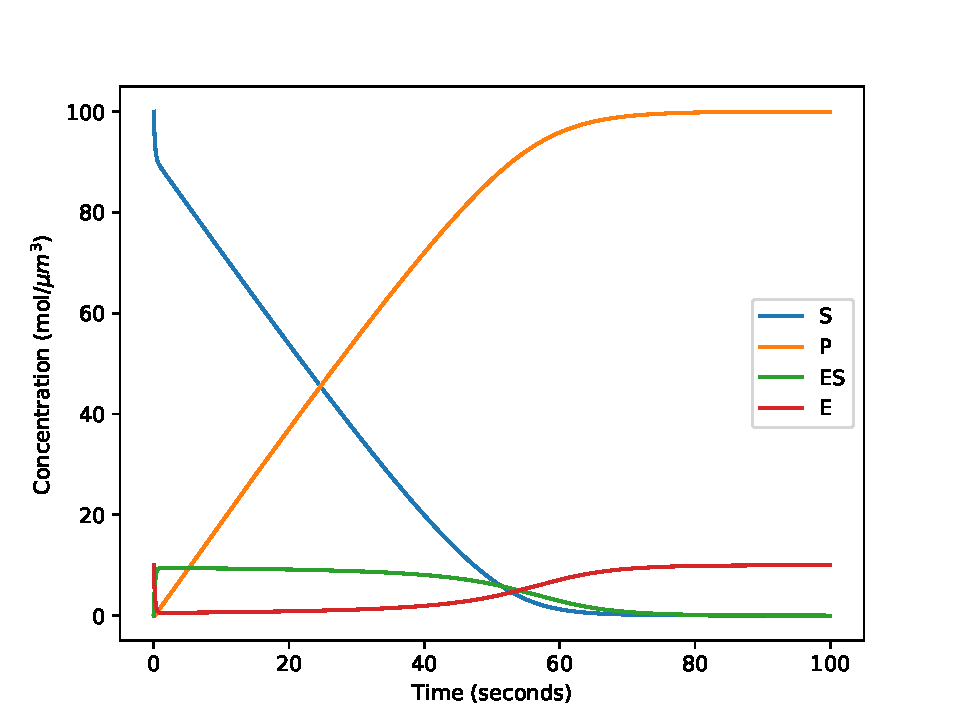
\includegraphics[trim={0 0 0 1.4cm}, clip=true, width=.45\textwidth]{fundamental_concepts/simplifications/full_system.pdf}}
     \label{fig:enzymatic_full}}
     &
    \subfigure[] {\scalebox{1}{
    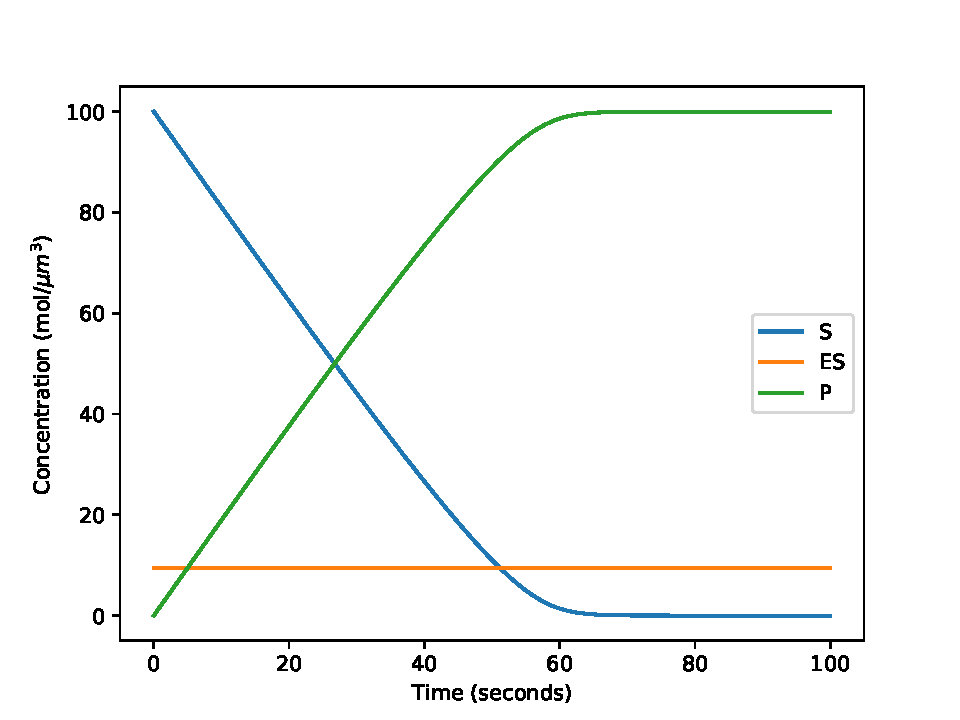
\includegraphics[trim={0 0 0 1.4cm}, clip=true, width=.45\textwidth]{fundamental_concepts/simplifications/mm_system.pdf}}
    \label{fig:enzymatic_mm}}
  \end{tabular}
    \caption{An example of the dynamics produced by two models of 
        enzymatic reactions. The Figure~\ref{fig:enzymatic_full} 
        presents the dynamics of the model~\ref{eq:full_system} and 
        Figure~\ref{fig:enzymatic_mm} presents the dynamics of the 
        Michaelis-Menten simplification to the same model. For this 
        simulations, it is necessary to define initial concentrations of
        the chemical species involved, and it is used: 
        10 molecules$/(\mu m)^3$ for the enzyme (E); 
        100~molecules$/(\mu m)^3$ is used for the substrate (S); and 
        0~molecules$/(\mu m)^3$ is used for the other species. In 
        addition to this, it is also necessary to define model 
        parameter values, and it is used: 
        0.06~$(\mu m)^3$(molecules$*s)^{-1}$ for $k_f$; 
        0.1~$(s^{-1})$ for $k_r$; 0.2~($s^{-1}$) for $k_{cat}$; and,
        following the Michalis-Menten model, 5 molecules$/(\mu m)^3$
        is used for $K_m$.}
  \label{fig:michaelis_menten} 
\end{figure}

% What to talk about:
% 1. Define identification of cell signaling pathways
%    -> Identification of signaling pathways is the problem of finding 
%       the components of a signaling network and how they interact 
%       in order to reproduce some behaviour of the cell that was
%       previously measured experimentally. 
%    -> The input of the problem should be then a description of the 
%       biological experiment and the measurements made on this 
%       experiment. As an output, we are expected to give a topology
%       of the network of interactions that are actively controlling
%       the cell behaviour observed on experiment measurements. More 
%       than that, we are also supposed to determine the set of 
%       parameter values that should be used on the models to reproduce
%       measurements similar to the experiments (or a probability 
%       distribution).
%    -> Two main tasks onto creating the output: you have to find 
%       a topology that is good with some parameter to reproduce the 
%       experiment; note that these tasks are very strongly correlated
%       and should be done together. 
% 2. Explain the challenges of cell signaling pathways
%    -> Firstly, simulating these problems is very time-consuming (even 
%       tough there are many ode solvers out there)
%    -> The number of possible interactions is very big. If we consider
%       choosing from n interactions a subset of them that should be on 
%       the topology, then there are 2^n options.
%    -> Once you choose two candidates of topology, it is still hard to
%       tell which one is better.
% (?). Talk about the work of Marcelo. State that current solutions do
%       not systematically search for the solution. 
% 3. somehow link to the next section, about cost functions 
%    -> Many of the state of the art approaches on identification of 
%       cell signaling network are based on a Bayesian approach for 
%       model ranking.
\section{Identification of Cell Signaling Pathways}
Identification of signaling pathways is the problem of finding the 
components of a signaling pathway and how they interact in order to
reproduce a behaviour of the cell that has been previously measured 
experimentally. The input of this problem is usually a description of 
the biological experiment, containing previous information about the 
signaling pathway, and a set of measurements, commonly Western blot 
data. The output to this problem is then composed of a set of 
interactions that are actively controlling the behaviour of interest of 
the cell, and also the set of parameter values that should be used on 
these interactions to create a model that approximates the experimental 
observations; it is possible to output a single value for each 
parameter, as it was presented in~\cite{Wu15}, or output information 
about these values, using a posterior (to the experimental data) 
distribution, as it was presented in~\cite{Liepe2014}~and~\cite{Xura20}.

Two main tasks must be completed to produce this output. The first task
is to find candidate topologies for the pathway model, i.e. different
set of interactions that are relevant to the pathway of interest. The
second task is to rank those models according to their ability to 
simulate the pathway and approximate the experimental measurements.

% To the second task, you can use combinatorics optimization to fit the
% model to the data and calculate the distance of the measurements on 
% the fitted model to the experimental data; then it is possible to rank
% models according to this distance. Alternatively, it is 
% possible to consider that the model parameters are random variables 
% and calculate the marginal probability of the model to reproduce the 
% observed data; then, it is possible to rank models according to this 
% probability.

The second task is also known as the model selection problem and even
though it is a broad area, there are works on the literature that treats 
specifically the problem in a biochemical context. Solutions to this 
problem should be able to choose model candidates according to their 
ability to reproduce observed data and penalize overly complex models 
to avoid overfitting. 

One approach on setting the score of a model is to search for the set of 
parameter values that makes the model measurements the closest to the 
experimental data and then define a distance between these two 
measurements; then it is possible to use this distance plus a penalty 
for complexity to create a ranking of the models. We can write this 
scoring function as:
\begin{equation*}
    score_1 (M) = - min_{\{\theta \in \Theta' \subset \Theta\}}  
        dist (\phi(M, \theta), D) + R (M),
\end{equation*}
where $M$ is the model, $\Theta$ is the parameter space, $\Theta'$ is 
the subset of the parameter space where the search for the best 
parameter values was conduced, $D$ is the experimental measurement,
$\phi$ is a function that determines the simulated measurement on the 
model, and $R$ is a regularization function that penalizes model 
complexity. This approach was implemented on the work of Lulu 
Wu~\cite{Wu15}, using a Simulated Annealing procedure to search for 
parameter values that minimizes the distance between simulation and 
experiment. The Simulated Annealing procedure used is available on the 
software SigNetSim (Signaling Network Simulator), which is based on the
of the work of Chu on~\cite{Chu1999}. However, Wu's methodology showed 
limitations when testing the ability to reconstruct models from 
experiments, and this could be related to the used penalization term. 
In fact, choosing a good regularization function is crucial to the 
performance of this methodology.

Another approach is to consider the model parameters as random variables 
and then marginalize the probability of the model and parameters to 
reproduce the observed data, i.e. estimate (because calculating is 
usually hard) the marginal probability:
\begin{equation}
    p (D | M) = \int_{\Theta} p (D | M, \theta) p (\theta | M) d\theta,
    \label{eq:marginal_likelihood_integral}
\end{equation}
where $D$ is the observed data, $M$ is the model and $\Theta$ is the 
parameter space. The function $p(\theta | M)$ is the prior probability 
function of the parameter $\theta$ on model $M$ and the function 
$p (D | M, \theta)$ is the likelihood of observing the data $D$ when
simulating the model $M$ using parameters $\theta$. Sometimes, however,
the likelihood function is unknown or computationally intractable; for
these cases, it is possible to use an alternative Bayesian approach, 
called Aproximate Bayesian Computation (ABC), to estimate the 
probability $p (M | D)$ and use it as a ranking score~\cite{Toni2009}.

% However, to the first task, there are not many methods on the 
% literature to solve this problem. Generally, this is solved using 
% both interactome maps from KEGG and the prior knowledge of the 
% researchers.
For the first task of identification of signaling pathways we described, 
the creation of model candidates, there are not as many works on the 
literature as there are for the second task. Commonly, researchers must 
resort on their own knowledge on the biological experiment and consult 
interactome maps available on repositories such as KEGG and BioModels to
construct manually the hypothesis of models for a signaling pathway. 
That enlightens the importance to create a methodology that 
systematically creates candidate models of signaling networks, as we 
propose on this project.



% What are the best approaches on model selection recently
% -> Most of them uses Bayesian ideas
% -> good because they can provide statistical formality about the 
%    selection.
% -> automatic penalization; allows researcher to introduce biological
%    information through the priors.
% -> it makes sense that a parameter is a random variable
% -> Explain BIBm
% -> Explain ABC-SysBio
% -> Even though they provide ways of ranking models, they don't treat
% the modeling of the network topology.
% -> Bayesian approaches
\section{State of the Art in Selection of Biochemical Models}
The state of the art in biochemical model selection is based on Bayesian
inference. The Bayesian approaches provide the benefits of ranking 
models with statistical formalism, and automatically penalizes overly 
complex models. More than that, through the prior distribution of the
parameters, the researcher is able to input prior knowledge about 
interactions constants; this type of information can facilitate the 
parameter inference of models since it tends to concentrate the search.

Bayesian approaches consider that model parameters are random variables, 
instead of fixed unknown constants. We can argue that this modeling is 
fair to the reality in biochemical processes because interactions 
constants can vary depending on the cell conditions. Therefore, in a 
biological experiment in which there might be perturbations to the cell 
environment, it should be more adequate to rank models integrating the 
models score over a probability space of parameters instead of fitting 
the model to data using a single point of the parameter space. We will 
now present the basic concept of two methods that use this idea for 
model selection, the Annealing-Melting Integration 
(AMI)~\cite{Vyshemirsky2007} and Approximate Bayesian Computation 
(ABC)~\cite{Toni2009}.

% What to mention about AMI:
% -> thermodynamic integral
% -> we are estimating the log of p(D|M, theta)
% -> theta being distributed according to some q_beta (\theta)
% -> q_beta are bridging distributions from prior to posterior
% -> to estimate this integral we need to use Monte Carlo Markov Chains
The Annealing-Melting Integration is a method that estimates the 
integral~\ref{eq:marginal_likelihood_integral} using concepts of 
thermodynamics. With thermodynamic integration, it is possible to write 
the logarithm of this integral as:
\begin{equation}
        \ln p(D|M) 
            = \int_0^1 \expectation_{q_\beta(\theta)} 
              [\ln p(D | M, \theta)] d\beta
        \label{eq:thermodynamic_integral}
\end{equation}
where $p(D|M,\theta)$ is the likelihood function (the 
probability of observing the data D when $M$ is the correct model, with
parameters $\theta$); and $\expectation_{q_\beta (\theta)}$ is an 
expectation taken over the probability space of $q_\beta(\theta) 
\propto p(D|M, \theta)^\beta p(\theta|M)$. The 
variable $\beta$ works in the integral as a temperature term, 
determining the probability functions $q_{\beta}(\theta)$; note that 
when $\beta = 0$ then 
\begin{equation*}
q_0(\theta) = p(\theta|M),
\end{equation*}
the prior distribution of the parameters, and when 
$\beta = 1$ then 
\begin{equation*}
    q_1(\theta) = \frac{p(D, \theta| M)} {\int_{\Theta}
                            p(D, \theta| M)} 
                = \frac{p(\theta | D, M)p(D|M)} 
                        {p(D | M)}
                = p(\theta | D, M),
\end{equation*}
the posterior distribution of parameters. Therefore, the 
integral~\ref{eq:thermodynamic_integral} takes the expected value of the
likelihood function of $D$ over a sequence of probability distributions
that is a ``bridge of distributions'' connecting the prior and posterior 
distributions of parameters. Calculating the integral is usually 
infeasible, hence in practice it is needed to estimate this integral 
using samples of a finite number of tempered distributions, 
$q_\beta(\theta)$.

% How about ABC?
% -> Likelihood free!
% -> Define the algorithm
%   -> The goal of the algorithm is to find a ``good" sample of 
%      parameters for the observed data.
%   -> The algorithm proposes a candidate parameter \theta*.
%   -> Simulate the model with those parameters.
%   -> Using a distance function d, accept theta* if
%      d(simulation, data) < eps
As we mentioned before, the likelihood function 
$p(D | M, \theta)$ may be very hard to calculate if not 
impossible. For those cases it is possible to use parameter inference
approaches that are likelihood-free, called Approximate Bayesian 
Computation (ABC). This method has the goal of producing a sample of 
parameters that brings the model simulations close to the observed data.
A generic ABC algorithm starts proposing a candidate parameter 
$\theta^*$ from a proposal distribution; then, a simulation, 
$\phi (M, \theta^*)$ of the model using the candidate parameters is 
produced; if, for some distance function $d$, is true that 
$d(\phi(M, \theta^*), D) < \epsilon$, then we accept $\theta^*$ as part
of the sample. If $\epsilon$ is sufficiently small, then the produced
samples approximates well the posterior distribution. To use ABC methods
for model selection it is enough to add a model indicator parameter to 
the parameter array, then it is possible to extract model distribution
of the accepted parameters.

% Metropolis-Hastings algorithm
% -> Both methods for model selection, based on ABC or using 
% thermodynamics integration needs to generate samples of probability 
% distributions. Generating samples of distributions is easy for many 
% well known distributions, however, for some other distributions it may
% not simple. 
% -> What does it do?
% Metropolis-Hastings algorithms are capable of generating a
% sample that has some probability distribution $p$, the target 
% function. The method can be used even when it is not possible to 
% calculate points of the target probability function, because all it is
% needed is a function that is proportional to the target. This is 
% useful for example when the target function is a posterior
% -> How do we do this
%   -> 
\section{Metropolis-Hastings to Generate Samples}
Both methods for model selection, based on ABC or using thermodynamics
integration need to generate samples of probability distributions. 
Generating samples of distributions is simple for many well known 
distributions, however, for some other distributions it may not be as
simple. Metropolis-Hastings algorithms are capable of generating a 
sample that has some probability distribution $p$, which is called the 
target distribution. In fact, the method can be used even when it is not
possible to access directly the target function, because all it is 
needed to perform the sampling is a function that is proportional to the
target.

Being able to generate a sample of a target distribution without 
accessing the probability function itself is useful for our applications
in Bayesian model ranking. Consider that we need to create a sample of
the parameters posterior distribution $p (\theta | M, D)$. Calculating 
this probability function is very hard because
\begin{equation*}
    p(\theta | M, D) = \frac{p (D | \theta, M) p (\theta | M)}
                            {p (D|M)},
\end{equation*}
and this equation has the term $p (D|M)$, which is only known (by some 
estimation) at the end of the model ranking; however, if we can access
the likelihood function $p (D| \theta, M)$ and the prior 
$p (\theta | M)$ than the product of these two is proportional to the 
posterior distribution (since $p (D|M)$ is only a constant because it
does not depend on $\theta$), and therefore they are enough to generate
a sample of the posterior.

A generic Metropolis-Hastings algorithm that creates a sample of a 
target distribution $p (\lambda)$ proceeds as follows:
\begin{enumerate}
\item{Choose some starting point $\lambda_0$ for which $p (\lambda_0)$ 
    is not zero. Also set $t = 1$.}
\item{Sample a candidate point $\lambda^*$ from a proposal (or jumping) 
    distribution with probability $J_t (\lambda^* | \lambda^{t - 1})$.}
    \label{enum:iteration_start}
\item{Calculate the ratio:}
    \begin{equation}
        r = \frac{p (\lambda^*) J_t (\lambda^{t - 1} | \lambda^*)}
                 {p (\lambda^{t - 1}) J_t (\lambda^* | \lambda^{t - 1})}
        \label{eq:mh_ratio}
    \end{equation}
\item{With probability $min (1, r)$ set $\theta^t = \theta^*$ and set
    $\theta^t = \theta^{t - 1}$ otherwise.}
\item{Increase $t$ by one and, if not reached limit number of 
    iterations, go back to step~\ref{enum:iteration_start}.}
\end{enumerate}
Note that if the target $p (\lambda)$ is not available, and rather 
another function $q (\lambda) = \frac{1}{c}p(\lambda)$ is available, 
then the ratio~\ref{eq:mh_ratio} can be calculated as:
\begin{equation*}
    r = \frac{p (\lambda^*) J_t (\lambda^{t - 1} | \lambda^*)}
              {p (\lambda^{t - 1}) J_t (\lambda^* | \lambda^{t - 1})} 
      = \frac{(q (\lambda^*)c) J_t (\lambda^{t - 1} | \lambda^*)}
           {(q (\lambda^{t - 1})c) J_t (\lambda^* | \lambda^{t - 1})} 
      = \frac{q (\lambda^*) J_t (\lambda^{t - 1} | \lambda^*)}
              {q (\lambda^{t - 1}) J_t (\lambda^* | \lambda^{t - 1})}
\end{equation*}
More than that, if the proposal distribution is symmetric, the produced 
algorithm is called Metropolis algorithm and has the ratio 
$r = {p (\lambda^*)}/{p (\lambda^{t - 1})}$. 

Different implementations of the Metropolis-Hastings algorithm are 
possible. The possible changes include the choice of starting point,
the choice of proposal distributions and number of iterations. As an
example, some algorithms are adaptive in the sense that they can change 
the proposal distribution according to the acceptance rate of proposed 
points~\cite{Gelman2013}.


\chapter{Model Selection Methods}
\label{chap:model_selection}
%begin-include
{\color{blue} Simple description of the content of this chapter}.

\section{Model ranking using Marginal Likelihood}
% Simple explanation of this model ranking
% Describe the likelihood function 
% However, this is very hard to calculate
% It is possible to apply an Importance Sampling Estimator {cite 
% Newton and Raftery}. However, it was showed on {cite girolami again}
% that these methods do not perform well.
% Then it was proposed to use Thermodynamic Integration. Make it clear 
% that this allows us to create some estimators.
% Subsection - Thermodynamic Integration
% -> explain how to derive it
%   -> name what is the power posterior
% -> include here: how to estimate it?
% Subsection - Estimation of the Marginal Likelihood 
% -> We need to find samples of the posteriors
% -> Explain that we use the methodology of Xuan
% -> We use three Metropolis-Hastings
% -> A first burn-in step with jumps independent for each single 
% parameter. Adaptive Metropolis Hastings
% -> A second using a Variance-Covariance Matrix
% -> A third using populational MCMC
The marginal likelihood of an experiment measurement $D$ being 
reproduced by a model $M$, $p (D | M)$, can be used as a model ranking 
metric as it determines which model makes the experimental observations 
more likely to happen. Before defining how to calculate the  marginal 
the likelihood, we must define what the likelihood function is. To 
calculate the likelihood $p (D | M, \theta)$, we must understand that 
conditioning the observation to the model and parameters means that in 
the probability space from which $D$ is taken, the model $M$ is the 
``real'' model and it has the parameter values of $\theta$; i.e. the 
model $M$ with parameters $\theta$ controls the behaviour of the system 
from which $D$ was observed. Then, assuming that the observations have a 
Gaussian error, and that they are taken in a time series of $m$ time 
steps, we can define the likelihood as:
\begin{equation}
    p (D | M, \theta) = p_{\mathcal{N}_{\left(\vec{0}, \Sigma\right)}}
        (\phi (M,\theta) - D),
\label{eq:likelihood_multivariate}
\end{equation}
where $\phi (M, \theta) \in \fieldR^m$ is the experimental measurement 
on the simulation generated by the model $M$ with parameters $\theta$,
and \smash{$p_{\mathcal{N}_{(\vec{0}, \Sigma)}} (\cdot)$} is the 
probability density function of a Multivariate Normal variable with mean 
$\vec{0}$ and covariance matrix $\Sigma$. As a matter of fact, as it is
done in the work of Xu et al., we can consider that the observation 
error is independent for each time step~\cite{Xura20}, therefore we can 
simplify~\ref{eq:likelihood_multivariate} to:
\begin{equation}
    p (D | M, \theta) = \prod_{i = 1}^m p_{\mathcal{N}_{\left(0, 
        \sigma^2\right)}} (\phi_i (M,\theta) - D_i).
\label{eq:likelihood}
\end{equation}
The $\sigma^2$ used in equation~\ref{eq:likelihood} is also a parameter
of the model, which means that, for some $k$, $\theta_k = \sigma^2$.

Now that we defined the likelihood function, we can write the marginal 
likelihood as:
\begin{equation}
    p (D | M) = \int_{\Theta} p (D | M, \theta) p (\theta | M)d\theta.
\label{eq:marginal_likelihood}
\end{equation}
However, calculating this integral analytically is only possible in 
very special cases and, usually, it would depend on knowing models for 
the distributions associated to these probability functions, which is 
generally not possible in our case.

Even though this integral is very hard to be calculated, there are 
methods that allow us to estimate its value. A straight forward method 
to estimate this integral value is the Importance Sampling 
Estimator~\cite{Newton1993}. This method uses the Monte Carlo integral 
estimation method that can estimate integrals of the form 
$\int g(\lambda) p(\lambda)d\lambda$ using the estimator:
\begin{equation}
    \hat{I} = \sum_{i = 1}^m w_i g(\lambda_i) / \sum_{i = 1}^m w_i,
\label{eq:importance_sampling_estimator}
\end{equation}
where $w_i = p (\lambda) / p^* (\lambda)$, and $p^*(\cdot)$ is known as 
the importance sampling function. If we set $\lambda = \theta | M$ and
use the prior ($p(\theta | M)$) or the posterior ($p(\theta | M, D)$) as 
importance sampling functions, then we would get respectively the 
estimators:
\begin{equation}
\begin{aligned}
    \frac{1}{m} \sum_{i = 1}^m p(D|M, \theta^{(i)}) &&& 
        (\text{with } \theta^{(i)} \sim p(\theta|M)); \\
    \left(\frac{1}{m} \sum_{i = 1}^m p(D|M, \theta^{(i)})^{-1} \right)^{-1} &&&
        (\text{with } \theta^{(i)} \sim p(\theta|M)).
\end{aligned}
\end{equation}
However, as showed by Vyshemirsky et al. (2007), these estimators might
produce very large variances and may not perform well for biochemical
model selection applications. For that reason we decide to use a 
Annealing-Melting method as it is proposed in the same 
work~\cite{Vyshemirsky2007}.

% ABC-SysBio
% Experiments comparing both approaches


\chapter{Experiments on Model Selection}
\label{chap:exp_on_model_selection}
%begin-include
\section{Software for Ranking of Models of Signaling Networks}
In this section we describe the software we used to perform the ranking
of signaling network models. The first software, SigNetMS, is an 
implementation of the model ranking method presented on 
section~\ref{sec:marginal_likelihood_method}, which estimates the 
marginal likelihood of the data being reproduced by a model.  The second 
software, ABC-SysBio implements the method based on the approximate 
Bayesian Computation, presented on section~\ref{sec:abc_method}.

\subsection{SigNetMS}
To perform the model ranking using an estimate of the marginal 
likelihood, we created the software SigNetMS, which is an acronym of 
{\bf Sig}naling {\bf Net}work {\bf M}odel {\bf S}election. This software
was implemented in Python and it is a free software, under the \emph{GNU 
General Public License}, and available on
\href{https://github.com/gustavoem/SigNetMS}{GitHub}. The SigNetMS 
software can read and parse files containing models of signaling network 
represented in the Systems Biology Markup Language (SBML) format and 
then construct the respective system of differential equations according 
to the chemical species and interactions defined on the file. The 
experiments observations and prior distributions of parameters are 
defined by the user with Extensible Markup Language (XML) files. Four 
other parameters are necessary to run SigNetMS, all of them related to 
the sampling of the power posteriors. 

The method we used to sample each of the power posterior distributions
is the one we presented on section~\ref{sec:power_posteriors_sampling}.
The four parameters related to the sampling determine the size of all
sampling  performed and also the adaptive behaviour of one of the 
Metropolis-Hastings algorithm used. The first parameter defines the 
number of iterations of the first sampling algorithm. This algorithm is 
adaptive because, after a fixed number of iterations, the covariance of 
the jump distribution is updated according to the acceptance rate of 
proposed points; this fixed number of iterations is the second sampling 
parameter. Finally, the third and fourth parameter determine the size of
the second and third sampling steps respectively.

To implement the method we still have to define the proposal 
distributions. Since the proposed model parameters cannot have 
nonpositive values (because they are reaction rate constants), the 
proposal distribution should have a probability density function that 
has value zero for nonpositive numbers. Moreover, its desired, through 
the sampling steps, to control the mean and variance of the proposal 
distributions. For all of the three steps, if the current point of the
chain is $\theta$, then the jump distribution should have mean close
to $\theta$. Also, in the first step, the covariance matrix  of the 
proposal distribution should be proportional to the covariance of 
the prior distribution of parameters. Then, for the two final steps, the 
covariance matrix of the jump distribution should be proportional to an
estimate $\hat{C}$ of the covariance of the parameters, calculated with 
the accepted points of the chain.

In our first attempt, we used multivariate lognormal distributions for 
all the sampling steps. If $X$ is a $MultivariateNormal (\mu, \Sigma)$, 
then $Y = e^{X}$ is $MultivariateLognormal (\mu, \Sigma)$. However, we 
found out that for some combinations of $\theta$ and $\hat{C}$, there 
is no combination of parameters $(\mu, \Sigma)$ such that $Y \propto 
MultivariateLognormal (\mu, \Sigma)$ with $\expectation[Y] = \theta$ and
$var(Y) = \hat{C}$. Then the solution we proposed is to use a truncated 
normal distribution for which only positive numbers have positive 
probability. We can generate a truncated normal random variable, 
$Y \propto TruncatedNormal (\mu, \Sigma)$ by 
repeatedly generating a normal random variable, $X \propto Normal(\mu, 
\Sigma)$ until $X$ is positive. However, this approach has the drawback 
that  $\expectation[Y]$ is usually greater than $\mu$, implying on a 
biased run of Metropolis-Hastings.
{\color{blue} Maybe we should state here that we can't calculate pdf of
the truncated normal distribution?}

The SigNetMS program also has an optional argument that allows the user
to get a verbose run, showing all proposed parameters for each 
temperature as well as the accepted parameters used to estimate the 
logarithm of the marginal likelihood. 

%-> implemented in Python
%-> implements the ABC-SMC method we explained earlier
%-> also reads models in SBML format
\section{ABC-SysBio}
ABC-SysBio is a Python software that implements the Approximate Bayesian
Computation Sequential Monte Carlo (ABC SMC) method~\cite{Liepe2010}. 
This software, similarly to SigNetMS, also takes as input SBML models as 
well as prior distribution of parameters and experimental data. As the 
output, the software returns, for each candidate model, an estimate of 
the probability of that model reproducing the experimental data. The 
source code of the method is available on 
\href{https://sourceforge.net/projects/abc-sysbio/files/}{SourceForge}.

\section{Model Selection Experiments}
The experiments we performed to test both methods consists in taking 
four candidate models and ranking them according to experimental data 
generated by one of them.

\section{Results}




\chapter{Future Activities}
\label{chap:future_activities}
%begin-include
As we presented of the last sections of this text, we are close to
defining a ranking framework for models of signaling pathway. To achieve
our goal, of creating a methodology for identification of signaling 
pathway using an approach based on the feature selection problem, a few
activities need to be accomplished. These activities include the
definition of a reliable method of model ranking, the construction of
a relational database with chemical reactions information, the creation
of search algorithms in the space of models, and finally the validation
of the proposed methodology.

The first activity that should be tackled is the definition of a 
framework for ranking models of signaling pathways. This framework will
use either the ABC-SysBio or SigNetMS software. The first has been 
tested already and the last is still being tested and analyzed. 
Therefore, to define the framework we need to finish the tests of 
SigNetMS and decide which software is more adequate for our use. After
that, it is of our interest to propose changes in the implementation of 
the chosen software in order to achieve better computational times, 
using, as an example, distributed computation or computation in multiple 
processors, including graphics processing units (GPUs).

After defining the model ranking framework, we will define the 
relational database of chemical reactions, which will be used to define 
the search space of the feature selection problem. This database should
be able to store interactions between chemical species as well as 
reaction rate constants.  This database will be populated with 
information from other databases available, such as 
SABIO-RK~\cite{Wittig2011} and BRENDA~\cite{Schomburg2004}. Interactions 
of the database will be used to propose new model hypothesis for the 
experimental data, while the reaction rate constants will be used to 
define the prior distribution of model parameters (distributions should 
have high mass concentration around plausible values for reaction rate 
constants).

With a defined model ranking framework and a database with informations
of chemical reactions we will then work on the definition of the
search space and cost function that will allow us to solve the 
identification of signaling pathways as a feature selection problem.
The cost function should be implemented on featsel, a framework that 
will also allow us to implement and different search algorithms of 
feature selection that we create to solve our problem. The featsel
framework can also benchmark search algorithms, and this feature is 
going to be used by us to improve algorithms and choose the ones with 
better performance.

Using the cost function and search space that we defined on the featsel
framework

\section{Activities description}
\begin{itemize}
    \item{\bf Activity 1:} Finalize experiments with SigNetMS.
    \item{\bf Activity 2:} Determine, between ABC-SysBio and SigNetMS,
        which is best to rank models.
    \item{\bf Activity 3:} Studies of databases of chemical kinetics 
        such as SABIO-RK~\cite{Wittig2011} and 
        BRENDA~\cite{Schomburg2004}.
    \item{\bf Activity 4:} Creation of a relational database of chemical 
        interactions that is able to store the topology and rate 
        constants of reactions gathered from chemical kinetics 
        databases.
    \item{\bf Activity 6:} Implementation of a feature selection cost
        function and search space on featsel, which will allows us to 
        solve the identification of signaling pathways as a feature 
        selection problem.
    \item{\bf Activity 7:} Create new algorithms of feature selection
        for the problem of identification of signaling pathways.
    \item{\bf Activity 8:} Tests of the methodology developed on known
        pathways.
    \item{\bf Activity 9:} Aplication of the method in ERK signaling 
        pathways of tumor cell lines Y1 and HEK293.
\end{itemize}



\newpage
\printbibliography

\end{document}

